\batchmode
\documentclass[twoside]{book}

% Packages required by doxygen
\usepackage{fixltx2e}
\usepackage{calc}
\usepackage{doxygen}
\usepackage[export]{adjustbox} % also loads graphicx
\usepackage{graphicx}
\usepackage[utf8]{inputenc}
\usepackage{makeidx}
\usepackage{multicol}
\usepackage{multirow}
\PassOptionsToPackage{warn}{textcomp}
\usepackage{textcomp}
\usepackage[nointegrals]{wasysym}
\usepackage[table]{xcolor}

% Font selection
\usepackage[T1]{fontenc}
\usepackage[scaled=.90]{helvet}
\usepackage{courier}
\usepackage{amssymb}
\usepackage{sectsty}
\renewcommand{\familydefault}{\sfdefault}
\allsectionsfont{%
  \fontseries{bc}\selectfont%
  \color{darkgray}%
}
\renewcommand{\DoxyLabelFont}{%
  \fontseries{bc}\selectfont%
  \color{darkgray}%
}
\newcommand{\+}{\discretionary{\mbox{\scriptsize$\hookleftarrow$}}{}{}}

% Page & text layout
\usepackage{geometry}
\geometry{%
  a4paper,%
  top=2.5cm,%
  bottom=2.5cm,%
  left=2.5cm,%
  right=2.5cm%
}
\tolerance=750
\hfuzz=15pt
\hbadness=750
\setlength{\emergencystretch}{15pt}
\setlength{\parindent}{0cm}
\setlength{\parskip}{3ex plus 2ex minus 2ex}
\makeatletter
\renewcommand{\paragraph}{%
  \@startsection{paragraph}{4}{0ex}{-1.0ex}{1.0ex}{%
    \normalfont\normalsize\bfseries\SS@parafont%
  }%
}
\renewcommand{\subparagraph}{%
  \@startsection{subparagraph}{5}{0ex}{-1.0ex}{1.0ex}{%
    \normalfont\normalsize\bfseries\SS@subparafont%
  }%
}
\makeatother

% Headers & footers
\usepackage{fancyhdr}
\pagestyle{fancyplain}
\fancyhead[LE]{\fancyplain{}{\bfseries\thepage}}
\fancyhead[CE]{\fancyplain{}{}}
\fancyhead[RE]{\fancyplain{}{\bfseries\leftmark}}
\fancyhead[LO]{\fancyplain{}{\bfseries\rightmark}}
\fancyhead[CO]{\fancyplain{}{}}
\fancyhead[RO]{\fancyplain{}{\bfseries\thepage}}
\fancyfoot[LE]{\fancyplain{}{}}
\fancyfoot[CE]{\fancyplain{}{}}
\fancyfoot[RE]{\fancyplain{}{\bfseries\scriptsize Generated by Doxygen }}
\fancyfoot[LO]{\fancyplain{}{\bfseries\scriptsize Generated by Doxygen }}
\fancyfoot[CO]{\fancyplain{}{}}
\fancyfoot[RO]{\fancyplain{}{}}
\renewcommand{\footrulewidth}{0.4pt}
\renewcommand{\chaptermark}[1]{%
  \markboth{#1}{}%
}
\renewcommand{\sectionmark}[1]{%
  \markright{\thesection\ #1}%
}

% Indices & bibliography
\usepackage{natbib}
\usepackage[titles]{tocloft}
\setcounter{tocdepth}{3}
\setcounter{secnumdepth}{5}
\makeindex

% Hyperlinks (required, but should be loaded last)
\usepackage{ifpdf}
\ifpdf
  \usepackage[pdftex,pagebackref=true]{hyperref}
\else
  \usepackage[ps2pdf,pagebackref=true]{hyperref}
\fi
\hypersetup{%
  colorlinks=true,%
  linkcolor=blue,%
  citecolor=blue,%
  unicode%
}

% Custom commands
\newcommand{\clearemptydoublepage}{%
  \newpage{\pagestyle{empty}\cleardoublepage}%
}

\usepackage{caption}
\captionsetup{labelsep=space,justification=centering,font={bf},singlelinecheck=off,skip=4pt,position=top}

%===== C O N T E N T S =====

\begin{document}

% Titlepage & ToC
\hypersetup{pageanchor=false,
             bookmarksnumbered=true,
             pdfencoding=unicode
            }
\pagenumbering{alph}
\pagenumbering{arabic}
\hypersetup{pageanchor=true}

%--- Begin generated contents ---
\chapter{Demo problem\+: Solid Mechanics using unstructured meshes}
\label{index}\hypertarget{index}{}\hypertarget{index_q}{}\section{A few quick questions...}\label{index_q}
Since {\ttfamily oomph-\/lib} is developed as open-\/source software, any evidence that the code is being downloaded and used is very helpful for us as it helps to justify our continued work on this project.

We would therefore be extremely grateful if you could provide the information requested in the form below. Pressing the \char`\"{}submit\char`\"{} button will get you to the actual download page.

{\bfseries Note\+:} 
\begin{DoxyItemize}
\item All information will be treated as confidential. 
\item If you provide your email address and check the appropriate box we will add you to our mailing list to inform you of upgrades and bug fixes to the code. Rest assured that the mailing list is {\bfseries very low volume} -- we have better things to do than to bombard you with email. 
\item If you still feel reluctant to provide any of the information requested, feel free to enter some dummy input. The form will check that {\bfseries some} information has been entered but entering your name as \char`\"{}\+Joe Cool\char`\"{} is perfectly acceptable -- this is to discourage people from not providing the information simply because they are too lazy to type... 
\end{DoxyItemize}



 







 

 \hypertarget{index_pdf}{}\section{P\+D\+F file}\label{index_pdf}
A \href{../latex/refman.pdf}{\tt pdf version} of this document is available. \end{document}

\chapter{Namespace Index}
\section{Namespace List}
Here is a list of all namespaces with brief descriptions\+:\begin{DoxyCompactList}
\item\contentsline{section}{\hyperlink{namespaceGlobal__Physical__Variables}{Global\+\_\+\+Physical\+\_\+\+Variables} \\*Global variables that represent physical properties }{\pageref{namespaceGlobal__Physical__Variables}}{}
\item\contentsline{section}{\hyperlink{namespaceoomph}{oomph} }{\pageref{namespaceoomph}}{}
\item\contentsline{section}{\hyperlink{namespacePhysical__Variables}{Physical\+\_\+\+Variables} \\*Namespace for the solution of 2D linear shell equation }{\pageref{namespacePhysical__Variables}}{}
\end{DoxyCompactList}

\chapter{Hierarchical Index}
\section{Class Hierarchy}
This inheritance list is sorted roughly, but not completely, alphabetically\+:\begin{DoxyCompactList}
\item Problem\begin{DoxyCompactList}
\item \contentsline{section}{Unstructured\+Solid\+Problem$<$ E\+L\+E\+M\+E\+NT $>$}{\pageref{classUnstructuredSolidProblem}}{}
\end{DoxyCompactList}
\end{DoxyCompactList}

\chapter{Class Index}
\section{Class List}
Here are the classes, structs, unions and interfaces with brief descriptions\+:\begin{DoxyCompactList}
\item\contentsline{section}{\hyperlink{classPMLProblem}{P\+M\+L\+Problem$<$ E\+L\+E\+M\+E\+N\+T $>$} }{\pageref{classPMLProblem}}{}
\item\contentsline{section}{\hyperlink{classGlobalParameters_1_1TestPMLMapping}{Global\+Parameters\+::\+Test\+P\+M\+L\+Mapping} }{\pageref{classGlobalParameters_1_1TestPMLMapping}}{}
\end{DoxyCompactList}

\chapter{File Index}
\section{File List}
Here is a list of all files with brief descriptions\+:\begin{DoxyCompactList}
\item\contentsline{section}{\hyperlink{jeffery__orbit_8cc}{jeffery\+\_\+orbit.\+cc} }{\pageref{jeffery__orbit_8cc}}{}
\item\contentsline{section}{\hyperlink{jeffery__orbit_8txt__doxygenified_8h}{jeffery\+\_\+orbit.\+txt\+\_\+doxygenified.\+h} }{\pageref{jeffery__orbit_8txt__doxygenified_8h}}{}
\item\contentsline{section}{\hyperlink{my__taylor__hood__elements_8h}{my\+\_\+taylor\+\_\+hood\+\_\+elements.\+h} }{\pageref{my__taylor__hood__elements_8h}}{}
\end{DoxyCompactList}

\chapter{Namespace Documentation}
\hypertarget{namespaceGlobal__Physical__Variables}{}\section{Global\+\_\+\+Physical\+\_\+\+Variables Namespace Reference}
\label{namespaceGlobal__Physical__Variables}\index{Global\+\_\+\+Physical\+\_\+\+Variables@{Global\+\_\+\+Physical\+\_\+\+Variables}}


Namespace for physical parameters.  


\subsection*{Functions}
\begin{DoxyCompactItemize}
\item 
Vector$<$ double $>$ \hyperlink{namespaceGlobal__Physical__Variables_afae321364975eb56688ad13abc8ed6b7}{Gravity} (2)
\begin{DoxyCompactList}\small\item\em Gravity vector. \end{DoxyCompactList}\item 
void \hyperlink{namespaceGlobal__Physical__Variables_a87da705b8a46bed337cf5dbdd788b87b}{body\+\_\+force} (const double \&time, const Vector$<$ double $>$ \&x, Vector$<$ double $>$ \&result)
\begin{DoxyCompactList}\small\item\em Functional body force. \end{DoxyCompactList}\item 
void \hyperlink{namespaceGlobal__Physical__Variables_a9780d615ae07c4e00a436ab2973b54e6}{zero\+\_\+body\+\_\+force} (const double \&time, const Vector$<$ double $>$ \&x, Vector$<$ double $>$ \&result)
\begin{DoxyCompactList}\small\item\em Zero functional body force. \end{DoxyCompactList}\end{DoxyCompactItemize}
\subsection*{Variables}
\begin{DoxyCompactItemize}
\item 
double \hyperlink{namespaceGlobal__Physical__Variables_ab814e627d2eb5bc50318879d19ab16b9}{Re} =100
\begin{DoxyCompactList}\small\item\em Reynolds number. \end{DoxyCompactList}\item 
double \hyperlink{namespaceGlobal__Physical__Variables_ab1a845a672b4d74b304639a976dc65c6}{Re\+\_\+inv\+Fr} =100
\begin{DoxyCompactList}\small\item\em Reynolds/\+Froude number. \end{DoxyCompactList}\end{DoxyCompactItemize}


\subsection{Detailed Description}
Namespace for physical parameters. 

\subsection{Function Documentation}
\mbox{\Hypertarget{namespaceGlobal__Physical__Variables_a87da705b8a46bed337cf5dbdd788b87b}\label{namespaceGlobal__Physical__Variables_a87da705b8a46bed337cf5dbdd788b87b}} 
\index{Global\+\_\+\+Physical\+\_\+\+Variables@{Global\+\_\+\+Physical\+\_\+\+Variables}!body\+\_\+force@{body\+\_\+force}}
\index{body\+\_\+force@{body\+\_\+force}!Global\+\_\+\+Physical\+\_\+\+Variables@{Global\+\_\+\+Physical\+\_\+\+Variables}}
\subsubsection{\texorpdfstring{body\+\_\+force()}{body\_force()}}
{\footnotesize\ttfamily void Global\+\_\+\+Physical\+\_\+\+Variables\+::body\+\_\+force (\begin{DoxyParamCaption}\item[{const double \&}]{time,  }\item[{const Vector$<$ double $>$ \&}]{x,  }\item[{Vector$<$ double $>$ \&}]{result }\end{DoxyParamCaption})}



Functional body force. 



Definition at line 62 of file circular\+\_\+driven\+\_\+cavity.\+cc.



References Re\+\_\+inv\+Fr.



Referenced by main().

\mbox{\Hypertarget{namespaceGlobal__Physical__Variables_afae321364975eb56688ad13abc8ed6b7}\label{namespaceGlobal__Physical__Variables_afae321364975eb56688ad13abc8ed6b7}} 
\index{Global\+\_\+\+Physical\+\_\+\+Variables@{Global\+\_\+\+Physical\+\_\+\+Variables}!Gravity@{Gravity}}
\index{Gravity@{Gravity}!Global\+\_\+\+Physical\+\_\+\+Variables@{Global\+\_\+\+Physical\+\_\+\+Variables}}
\subsubsection{\texorpdfstring{Gravity()}{Gravity()}}
{\footnotesize\ttfamily Vector$<$double$>$ Global\+\_\+\+Physical\+\_\+\+Variables\+::\+Gravity (\begin{DoxyParamCaption}\item[{2}]{ }\end{DoxyParamCaption})}



Gravity vector. 



Referenced by main(), and Quarter\+Circle\+Driven\+Cavity\+Problem$<$ E\+L\+E\+M\+E\+N\+T $>$\+::\+Quarter\+Circle\+Driven\+Cavity\+Problem().

\mbox{\Hypertarget{namespaceGlobal__Physical__Variables_a9780d615ae07c4e00a436ab2973b54e6}\label{namespaceGlobal__Physical__Variables_a9780d615ae07c4e00a436ab2973b54e6}} 
\index{Global\+\_\+\+Physical\+\_\+\+Variables@{Global\+\_\+\+Physical\+\_\+\+Variables}!zero\+\_\+body\+\_\+force@{zero\+\_\+body\+\_\+force}}
\index{zero\+\_\+body\+\_\+force@{zero\+\_\+body\+\_\+force}!Global\+\_\+\+Physical\+\_\+\+Variables@{Global\+\_\+\+Physical\+\_\+\+Variables}}
\subsubsection{\texorpdfstring{zero\+\_\+body\+\_\+force()}{zero\_body\_force()}}
{\footnotesize\ttfamily void Global\+\_\+\+Physical\+\_\+\+Variables\+::zero\+\_\+body\+\_\+force (\begin{DoxyParamCaption}\item[{const double \&}]{time,  }\item[{const Vector$<$ double $>$ \&}]{x,  }\item[{Vector$<$ double $>$ \&}]{result }\end{DoxyParamCaption})}



Zero functional body force. 



Definition at line 70 of file circular\+\_\+driven\+\_\+cavity.\+cc.



Referenced by main().



\subsection{Variable Documentation}
\mbox{\Hypertarget{namespaceGlobal__Physical__Variables_ab814e627d2eb5bc50318879d19ab16b9}\label{namespaceGlobal__Physical__Variables_ab814e627d2eb5bc50318879d19ab16b9}} 
\index{Global\+\_\+\+Physical\+\_\+\+Variables@{Global\+\_\+\+Physical\+\_\+\+Variables}!Re@{Re}}
\index{Re@{Re}!Global\+\_\+\+Physical\+\_\+\+Variables@{Global\+\_\+\+Physical\+\_\+\+Variables}}
\subsubsection{\texorpdfstring{Re}{Re}}
{\footnotesize\ttfamily double Global\+\_\+\+Physical\+\_\+\+Variables\+::\+Re =100}



Reynolds number. 



Definition at line 53 of file circular\+\_\+driven\+\_\+cavity.\+cc.



Referenced by Quarter\+Circle\+Driven\+Cavity\+Problem$<$ E\+L\+E\+M\+E\+N\+T $>$\+::\+Quarter\+Circle\+Driven\+Cavity\+Problem().

\mbox{\Hypertarget{namespaceGlobal__Physical__Variables_ab1a845a672b4d74b304639a976dc65c6}\label{namespaceGlobal__Physical__Variables_ab1a845a672b4d74b304639a976dc65c6}} 
\index{Global\+\_\+\+Physical\+\_\+\+Variables@{Global\+\_\+\+Physical\+\_\+\+Variables}!Re\+\_\+inv\+Fr@{Re\+\_\+inv\+Fr}}
\index{Re\+\_\+inv\+Fr@{Re\+\_\+inv\+Fr}!Global\+\_\+\+Physical\+\_\+\+Variables@{Global\+\_\+\+Physical\+\_\+\+Variables}}
\subsubsection{\texorpdfstring{Re\+\_\+inv\+Fr}{Re\_invFr}}
{\footnotesize\ttfamily double Global\+\_\+\+Physical\+\_\+\+Variables\+::\+Re\+\_\+inv\+Fr =100}



Reynolds/\+Froude number. 



Definition at line 56 of file circular\+\_\+driven\+\_\+cavity.\+cc.



Referenced by body\+\_\+force(), and Quarter\+Circle\+Driven\+Cavity\+Problem$<$ E\+L\+E\+M\+E\+N\+T $>$\+::\+Quarter\+Circle\+Driven\+Cavity\+Problem().


\chapter{Class Documentation}
\hypertarget{classElasticTetMesh}{}\section{Elastic\+Tet\+Mesh$<$ E\+L\+E\+M\+E\+NT $>$ Class Template Reference}
\label{classElasticTetMesh}\index{Elastic\+Tet\+Mesh$<$ E\+L\+E\+M\+E\+N\+T $>$@{Elastic\+Tet\+Mesh$<$ E\+L\+E\+M\+E\+N\+T $>$}}


Triangle-\/based mesh upgraded to become a solid mesh.  


Inheritance diagram for Elastic\+Tet\+Mesh$<$ E\+L\+E\+M\+E\+NT $>$\+:\begin{figure}[H]
\begin{center}
\leavevmode
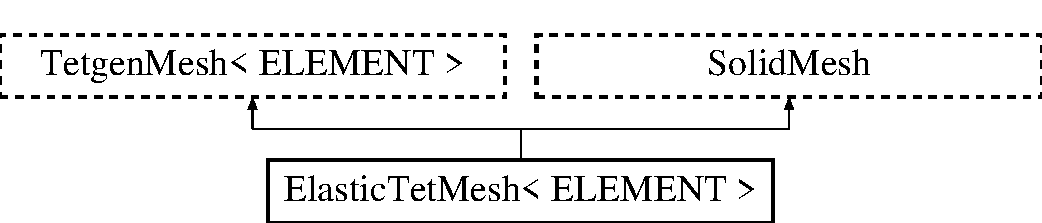
\includegraphics[height=2.000000cm]{classElasticTetMesh}
\end{center}
\end{figure}
\subsection*{Public Member Functions}
\begin{DoxyCompactItemize}
\item 
\hyperlink{classElasticTetMesh_afa0c8df37665c2b31b430de7e50dcc6b}{Elastic\+Tet\+Mesh} (const std\+::string \&node\+\_\+file\+\_\+name, const std\+::string \&element\+\_\+file\+\_\+name, const std\+::string \&poly\+\_\+file\+\_\+name, Time\+Stepper $\ast$time\+\_\+stepper\+\_\+pt=\&Mesh\+::\+Default\+\_\+\+Time\+Stepper)
\begin{DoxyCompactList}\small\item\em Constructor\+: \end{DoxyCompactList}\item 
virtual \hyperlink{classElasticTetMesh_a4d072ceb1fb8eb0d3d0f619e0221914c}{$\sim$\+Elastic\+Tet\+Mesh} ()
\begin{DoxyCompactList}\small\item\em Empty Destructor. \end{DoxyCompactList}\end{DoxyCompactItemize}


\subsection{Detailed Description}
\subsubsection*{template$<$class E\+L\+E\+M\+E\+NT$>$\newline
class Elastic\+Tet\+Mesh$<$ E\+L\+E\+M\+E\+N\+T $>$}

Triangle-\/based mesh upgraded to become a solid mesh. 

Definition at line 52 of file unstructured\+\_\+three\+\_\+d\+\_\+solid.\+cc.



\subsection{Constructor \& Destructor Documentation}
\mbox{\Hypertarget{classElasticTetMesh_afa0c8df37665c2b31b430de7e50dcc6b}\label{classElasticTetMesh_afa0c8df37665c2b31b430de7e50dcc6b}} 
\index{Elastic\+Tet\+Mesh@{Elastic\+Tet\+Mesh}!Elastic\+Tet\+Mesh@{Elastic\+Tet\+Mesh}}
\index{Elastic\+Tet\+Mesh@{Elastic\+Tet\+Mesh}!Elastic\+Tet\+Mesh@{Elastic\+Tet\+Mesh}}
\subsubsection{\texorpdfstring{Elastic\+Tet\+Mesh()}{ElasticTetMesh()}}
{\footnotesize\ttfamily template$<$class E\+L\+E\+M\+E\+NT$>$ \\
\hyperlink{classElasticTetMesh}{Elastic\+Tet\+Mesh}$<$ E\+L\+E\+M\+E\+NT $>$\+::\hyperlink{classElasticTetMesh}{Elastic\+Tet\+Mesh} (\begin{DoxyParamCaption}\item[{const std\+::string \&}]{node\+\_\+file\+\_\+name,  }\item[{const std\+::string \&}]{element\+\_\+file\+\_\+name,  }\item[{const std\+::string \&}]{poly\+\_\+file\+\_\+name,  }\item[{Time\+Stepper $\ast$}]{time\+\_\+stepper\+\_\+pt = {\ttfamily \&Mesh\+:\+:Default\+\_\+TimeStepper} }\end{DoxyParamCaption})\hspace{0.3cm}{\ttfamily [inline]}}



Constructor\+: 



Definition at line 59 of file unstructured\+\_\+three\+\_\+d\+\_\+solid.\+cc.

\mbox{\Hypertarget{classElasticTetMesh_a4d072ceb1fb8eb0d3d0f619e0221914c}\label{classElasticTetMesh_a4d072ceb1fb8eb0d3d0f619e0221914c}} 
\index{Elastic\+Tet\+Mesh@{Elastic\+Tet\+Mesh}!````~Elastic\+Tet\+Mesh@{$\sim$\+Elastic\+Tet\+Mesh}}
\index{````~Elastic\+Tet\+Mesh@{$\sim$\+Elastic\+Tet\+Mesh}!Elastic\+Tet\+Mesh@{Elastic\+Tet\+Mesh}}
\subsubsection{\texorpdfstring{$\sim$\+Elastic\+Tet\+Mesh()}{~ElasticTetMesh()}}
{\footnotesize\ttfamily template$<$class E\+L\+E\+M\+E\+NT$>$ \\
virtual \hyperlink{classElasticTetMesh}{Elastic\+Tet\+Mesh}$<$ E\+L\+E\+M\+E\+NT $>$\+::$\sim$\hyperlink{classElasticTetMesh}{Elastic\+Tet\+Mesh} (\begin{DoxyParamCaption}{ }\end{DoxyParamCaption})\hspace{0.3cm}{\ttfamily [inline]}, {\ttfamily [virtual]}}



Empty Destructor. 



Definition at line 102 of file unstructured\+\_\+three\+\_\+d\+\_\+solid.\+cc.



The documentation for this class was generated from the following file\+:\begin{DoxyCompactItemize}
\item 
\hyperlink{unstructured__three__d__solid_8cc}{unstructured\+\_\+three\+\_\+d\+\_\+solid.\+cc}\end{DoxyCompactItemize}

\hypertarget{classElasticTriangleMesh}{}\section{Elastic\+Triangle\+Mesh$<$ E\+L\+E\+M\+E\+NT $>$ Class Template Reference}
\label{classElasticTriangleMesh}\index{Elastic\+Triangle\+Mesh$<$ E\+L\+E\+M\+E\+N\+T $>$@{Elastic\+Triangle\+Mesh$<$ E\+L\+E\+M\+E\+N\+T $>$}}


Triangle-\/based mesh upgraded to become a (pseudo-\/) solid mesh.  


Inheritance diagram for Elastic\+Triangle\+Mesh$<$ E\+L\+E\+M\+E\+NT $>$\+:\begin{figure}[H]
\begin{center}
\leavevmode
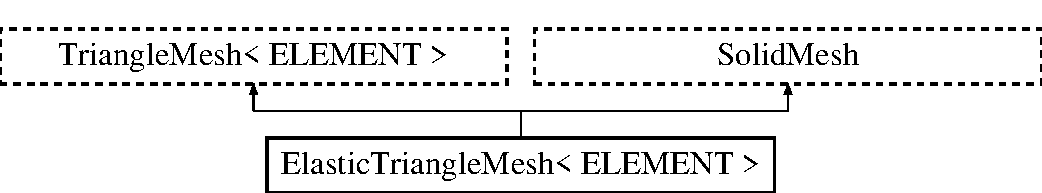
\includegraphics[height=2.000000cm]{classElasticTriangleMesh}
\end{center}
\end{figure}
\subsection*{Public Member Functions}
\begin{DoxyCompactItemize}
\item 
\hyperlink{classElasticTriangleMesh_a4c24e9abbde344d34e1e08fb3319d7b6}{Elastic\+Triangle\+Mesh} (const std\+::string \&node\+\_\+file\+\_\+name, const std\+::string \&element\+\_\+file\+\_\+name, const std\+::string \&poly\+\_\+file\+\_\+name, Time\+Stepper $\ast$time\+\_\+stepper\+\_\+pt=\&Mesh\+::\+Default\+\_\+\+Time\+Stepper)
\begin{DoxyCompactList}\small\item\em Constructor\+: \end{DoxyCompactList}\item 
void \hyperlink{classElasticTriangleMesh_aa83cad3dfdd980f95bf0dab6fd97bf22}{identify\+\_\+boundaries} ()
\begin{DoxyCompactList}\small\item\em Function used to identify the domain boundaries. \end{DoxyCompactList}\item 
virtual \hyperlink{classElasticTriangleMesh_ade80b912f1bb791e5f4fac35abf90504}{$\sim$\+Elastic\+Triangle\+Mesh} ()
\begin{DoxyCompactList}\small\item\em Empty Destructor. \end{DoxyCompactList}\end{DoxyCompactItemize}


\subsection{Detailed Description}
\subsubsection*{template$<$class E\+L\+E\+M\+E\+NT$>$\newline
class Elastic\+Triangle\+Mesh$<$ E\+L\+E\+M\+E\+N\+T $>$}

Triangle-\/based mesh upgraded to become a (pseudo-\/) solid mesh. 

Definition at line 52 of file unstructured\+\_\+two\+\_\+d\+\_\+fluid.\+cc.



\subsection{Constructor \& Destructor Documentation}
\mbox{\Hypertarget{classElasticTriangleMesh_a4c24e9abbde344d34e1e08fb3319d7b6}\label{classElasticTriangleMesh_a4c24e9abbde344d34e1e08fb3319d7b6}} 
\index{Elastic\+Triangle\+Mesh@{Elastic\+Triangle\+Mesh}!Elastic\+Triangle\+Mesh@{Elastic\+Triangle\+Mesh}}
\index{Elastic\+Triangle\+Mesh@{Elastic\+Triangle\+Mesh}!Elastic\+Triangle\+Mesh@{Elastic\+Triangle\+Mesh}}
\subsubsection{\texorpdfstring{Elastic\+Triangle\+Mesh()}{ElasticTriangleMesh()}}
{\footnotesize\ttfamily template$<$class E\+L\+E\+M\+E\+NT$>$ \\
\hyperlink{classElasticTriangleMesh}{Elastic\+Triangle\+Mesh}$<$ E\+L\+E\+M\+E\+NT $>$\+::\hyperlink{classElasticTriangleMesh}{Elastic\+Triangle\+Mesh} (\begin{DoxyParamCaption}\item[{const std\+::string \&}]{node\+\_\+file\+\_\+name,  }\item[{const std\+::string \&}]{element\+\_\+file\+\_\+name,  }\item[{const std\+::string \&}]{poly\+\_\+file\+\_\+name,  }\item[{Time\+Stepper $\ast$}]{time\+\_\+stepper\+\_\+pt = {\ttfamily \&Mesh\+:\+:Default\+\_\+TimeStepper} }\end{DoxyParamCaption})\hspace{0.3cm}{\ttfamily [inline]}}



Constructor\+: 



Definition at line 59 of file unstructured\+\_\+two\+\_\+d\+\_\+fluid.\+cc.

\mbox{\Hypertarget{classElasticTriangleMesh_ade80b912f1bb791e5f4fac35abf90504}\label{classElasticTriangleMesh_ade80b912f1bb791e5f4fac35abf90504}} 
\index{Elastic\+Triangle\+Mesh@{Elastic\+Triangle\+Mesh}!````~Elastic\+Triangle\+Mesh@{$\sim$\+Elastic\+Triangle\+Mesh}}
\index{````~Elastic\+Triangle\+Mesh@{$\sim$\+Elastic\+Triangle\+Mesh}!Elastic\+Triangle\+Mesh@{Elastic\+Triangle\+Mesh}}
\subsubsection{\texorpdfstring{$\sim$\+Elastic\+Triangle\+Mesh()}{~ElasticTriangleMesh()}}
{\footnotesize\ttfamily template$<$class E\+L\+E\+M\+E\+NT$>$ \\
virtual \hyperlink{classElasticTriangleMesh}{Elastic\+Triangle\+Mesh}$<$ E\+L\+E\+M\+E\+NT $>$\+::$\sim$\hyperlink{classElasticTriangleMesh}{Elastic\+Triangle\+Mesh} (\begin{DoxyParamCaption}{ }\end{DoxyParamCaption})\hspace{0.3cm}{\ttfamily [inline]}, {\ttfamily [virtual]}}



Empty Destructor. 



Definition at line 114 of file unstructured\+\_\+two\+\_\+d\+\_\+fluid.\+cc.



\subsection{Member Function Documentation}
\mbox{\Hypertarget{classElasticTriangleMesh_aa83cad3dfdd980f95bf0dab6fd97bf22}\label{classElasticTriangleMesh_aa83cad3dfdd980f95bf0dab6fd97bf22}} 
\index{Elastic\+Triangle\+Mesh@{Elastic\+Triangle\+Mesh}!identify\+\_\+boundaries@{identify\+\_\+boundaries}}
\index{identify\+\_\+boundaries@{identify\+\_\+boundaries}!Elastic\+Triangle\+Mesh@{Elastic\+Triangle\+Mesh}}
\subsubsection{\texorpdfstring{identify\+\_\+boundaries()}{identify\_boundaries()}}
{\footnotesize\ttfamily template$<$class E\+L\+E\+M\+E\+NT$>$ \\
void \hyperlink{classElasticTriangleMesh}{Elastic\+Triangle\+Mesh}$<$ E\+L\+E\+M\+E\+NT $>$\+::identify\+\_\+boundaries (\begin{DoxyParamCaption}{ }\end{DoxyParamCaption})\hspace{0.3cm}{\ttfamily [inline]}}



Function used to identify the domain boundaries. 



Definition at line 76 of file unstructured\+\_\+two\+\_\+d\+\_\+fluid.\+cc.



The documentation for this class was generated from the following file\+:\begin{DoxyCompactItemize}
\item 
\hyperlink{unstructured__two__d__fluid_8cc}{unstructured\+\_\+two\+\_\+d\+\_\+fluid.\+cc}\end{DoxyCompactItemize}

\hypertarget{classUnstructuredSolidProblem}{}\section{Unstructured\+Solid\+Problem$<$ E\+L\+E\+M\+E\+NT $>$ Class Template Reference}
\label{classUnstructuredSolidProblem}\index{Unstructured\+Solid\+Problem$<$ E\+L\+E\+M\+E\+N\+T $>$@{Unstructured\+Solid\+Problem$<$ E\+L\+E\+M\+E\+N\+T $>$}}


Unstructured solid problem.  


Inheritance diagram for Unstructured\+Solid\+Problem$<$ E\+L\+E\+M\+E\+NT $>$\+:\begin{figure}[H]
\begin{center}
\leavevmode
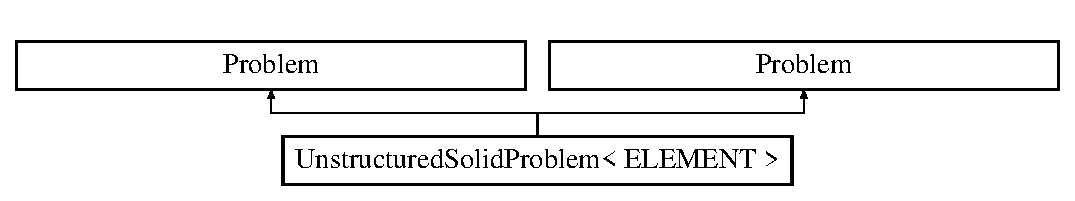
\includegraphics[height=2.000000cm]{classUnstructuredSolidProblem}
\end{center}
\end{figure}
\subsection*{Public Member Functions}
\begin{DoxyCompactItemize}
\item 
\hyperlink{classUnstructuredSolidProblem_a18ce02b6e4bbc86403c9e1b32c095772}{Unstructured\+Solid\+Problem} ()
\begin{DoxyCompactList}\small\item\em Constructor\+: \end{DoxyCompactList}\item 
\hyperlink{classUnstructuredSolidProblem_a25fe105d949498bf8f7c15aff96a7d00}{$\sim$\+Unstructured\+Solid\+Problem} ()
\begin{DoxyCompactList}\small\item\em Destructor (empty) \end{DoxyCompactList}\item 
void \hyperlink{classUnstructuredSolidProblem_ab3d66fd61b69d12b4f159d763fc44f15}{doc\+\_\+solution} (Doc\+Info \&doc\+\_\+info)
\begin{DoxyCompactList}\small\item\em Doc the solution. \end{DoxyCompactList}\end{DoxyCompactItemize}
\subsection*{Private Member Functions}
\begin{DoxyCompactItemize}
\item 
void \hyperlink{classUnstructuredSolidProblem_a9137960284200ed998989f785965f902}{create\+\_\+traction\+\_\+elements} ()
\begin{DoxyCompactList}\small\item\em Create traction elements. \end{DoxyCompactList}\end{DoxyCompactItemize}
\subsection*{Private Attributes}
\begin{DoxyCompactItemize}
\item 
\hyperlink{classMySolidTetgenMesh}{My\+Solid\+Tetgen\+Mesh}$<$ E\+L\+E\+M\+E\+NT $>$ $\ast$ \hyperlink{classUnstructuredSolidProblem_ad6a8cbe2c2f3596385e1a2484bfb68f7}{Solid\+\_\+mesh\+\_\+pt}
\begin{DoxyCompactList}\small\item\em Bulk solid mesh. \end{DoxyCompactList}\item 
Vector$<$ Solid\+Mesh $\ast$ $>$ \hyperlink{classUnstructuredSolidProblem_a32e691a698667053003e21333fc65057}{Solid\+\_\+traction\+\_\+mesh\+\_\+pt}
\begin{DoxyCompactList}\small\item\em Meshes of traction elements. \end{DoxyCompactList}\item 
Vector$<$ unsigned $>$ \hyperlink{classUnstructuredSolidProblem_a62ea7d593eaac6a3a0f0455c4a3fd805}{Pinned\+\_\+solid\+\_\+boundary\+\_\+id}
\begin{DoxyCompactList}\small\item\em I\+Ds of solid mesh boundaries where displacements are pinned. \end{DoxyCompactList}\item 
Vector$<$ unsigned $>$ \hyperlink{classUnstructuredSolidProblem_a4cf906bac719c9a942c04bda2798080f}{Solid\+\_\+traction\+\_\+boundary\+\_\+id}
\begin{DoxyCompactList}\small\item\em I\+Ds of solid mesh boundaries which make up the traction interface. \end{DoxyCompactList}\end{DoxyCompactItemize}


\subsection{Detailed Description}
\subsubsection*{template$<$class E\+L\+E\+M\+E\+NT$>$\newline
class Unstructured\+Solid\+Problem$<$ E\+L\+E\+M\+E\+N\+T $>$}

Unstructured solid problem. 

Definition at line 140 of file unstructured\+\_\+three\+\_\+d\+\_\+solid.\+cc.



\subsection{Constructor \& Destructor Documentation}
\mbox{\Hypertarget{classUnstructuredSolidProblem_a18ce02b6e4bbc86403c9e1b32c095772}\label{classUnstructuredSolidProblem_a18ce02b6e4bbc86403c9e1b32c095772}} 
\index{Unstructured\+Solid\+Problem@{Unstructured\+Solid\+Problem}!Unstructured\+Solid\+Problem@{Unstructured\+Solid\+Problem}}
\index{Unstructured\+Solid\+Problem@{Unstructured\+Solid\+Problem}!Unstructured\+Solid\+Problem@{Unstructured\+Solid\+Problem}}
\subsubsection{\texorpdfstring{Unstructured\+Solid\+Problem()}{UnstructuredSolidProblem()}}
{\footnotesize\ttfamily template$<$class E\+L\+E\+M\+E\+NT $>$ \\
\hyperlink{classUnstructuredSolidProblem}{Unstructured\+Solid\+Problem}$<$ E\+L\+E\+M\+E\+NT $>$\+::\hyperlink{classUnstructuredSolidProblem}{Unstructured\+Solid\+Problem} (\begin{DoxyParamCaption}{ }\end{DoxyParamCaption})}



Constructor\+: 

Constructor for unstructured solid problem. I\+Ds of solid mesh boundaries where displacements are pinned 

Definition at line 179 of file unstructured\+\_\+three\+\_\+d\+\_\+solid.\+cc.



References Global\+\_\+\+Parameters\+::\+Constitutive\+\_\+law\+\_\+pt, and Global\+\_\+\+Parameters\+::gravity().

\mbox{\Hypertarget{classUnstructuredSolidProblem_a25fe105d949498bf8f7c15aff96a7d00}\label{classUnstructuredSolidProblem_a25fe105d949498bf8f7c15aff96a7d00}} 
\index{Unstructured\+Solid\+Problem@{Unstructured\+Solid\+Problem}!````~Unstructured\+Solid\+Problem@{$\sim$\+Unstructured\+Solid\+Problem}}
\index{````~Unstructured\+Solid\+Problem@{$\sim$\+Unstructured\+Solid\+Problem}!Unstructured\+Solid\+Problem@{Unstructured\+Solid\+Problem}}
\subsubsection{\texorpdfstring{$\sim$\+Unstructured\+Solid\+Problem()}{~UnstructuredSolidProblem()}}
{\footnotesize\ttfamily template$<$class E\+L\+E\+M\+E\+NT$>$ \\
\hyperlink{classUnstructuredSolidProblem}{Unstructured\+Solid\+Problem}$<$ E\+L\+E\+M\+E\+NT $>$\+::$\sim$\hyperlink{classUnstructuredSolidProblem}{Unstructured\+Solid\+Problem} (\begin{DoxyParamCaption}{ }\end{DoxyParamCaption})\hspace{0.3cm}{\ttfamily [inline]}}



Destructor (empty) 



Definition at line 149 of file unstructured\+\_\+three\+\_\+d\+\_\+solid.\+cc.



\subsection{Member Function Documentation}
\mbox{\Hypertarget{classUnstructuredSolidProblem_a9137960284200ed998989f785965f902}\label{classUnstructuredSolidProblem_a9137960284200ed998989f785965f902}} 
\index{Unstructured\+Solid\+Problem@{Unstructured\+Solid\+Problem}!create\+\_\+traction\+\_\+elements@{create\+\_\+traction\+\_\+elements}}
\index{create\+\_\+traction\+\_\+elements@{create\+\_\+traction\+\_\+elements}!Unstructured\+Solid\+Problem@{Unstructured\+Solid\+Problem}}
\subsubsection{\texorpdfstring{create\+\_\+traction\+\_\+elements()}{create\_traction\_elements()}}
{\footnotesize\ttfamily template$<$class E\+L\+E\+M\+E\+NT $>$ \\
void \hyperlink{classUnstructuredSolidProblem}{Unstructured\+Solid\+Problem}$<$ E\+L\+E\+M\+E\+NT $>$\+::create\+\_\+traction\+\_\+elements (\begin{DoxyParamCaption}{ }\end{DoxyParamCaption})\hspace{0.3cm}{\ttfamily [private]}}



Create traction elements. 



Definition at line 301 of file unstructured\+\_\+three\+\_\+d\+\_\+solid.\+cc.



References Global\+\_\+\+Parameters\+::constant\+\_\+pressure().

\mbox{\Hypertarget{classUnstructuredSolidProblem_ab3d66fd61b69d12b4f159d763fc44f15}\label{classUnstructuredSolidProblem_ab3d66fd61b69d12b4f159d763fc44f15}} 
\index{Unstructured\+Solid\+Problem@{Unstructured\+Solid\+Problem}!doc\+\_\+solution@{doc\+\_\+solution}}
\index{doc\+\_\+solution@{doc\+\_\+solution}!Unstructured\+Solid\+Problem@{Unstructured\+Solid\+Problem}}
\subsubsection{\texorpdfstring{doc\+\_\+solution()}{doc\_solution()}}
{\footnotesize\ttfamily template$<$class E\+L\+E\+M\+E\+NT $>$ \\
void \hyperlink{classUnstructuredSolidProblem}{Unstructured\+Solid\+Problem}$<$ E\+L\+E\+M\+E\+NT $>$\+::doc\+\_\+solution (\begin{DoxyParamCaption}\item[{Doc\+Info \&}]{doc\+\_\+info }\end{DoxyParamCaption})}



Doc the solution. 



Definition at line 344 of file unstructured\+\_\+three\+\_\+d\+\_\+solid.\+cc.



Referenced by main().



\subsection{Member Data Documentation}
\mbox{\Hypertarget{classUnstructuredSolidProblem_a62ea7d593eaac6a3a0f0455c4a3fd805}\label{classUnstructuredSolidProblem_a62ea7d593eaac6a3a0f0455c4a3fd805}} 
\index{Unstructured\+Solid\+Problem@{Unstructured\+Solid\+Problem}!Pinned\+\_\+solid\+\_\+boundary\+\_\+id@{Pinned\+\_\+solid\+\_\+boundary\+\_\+id}}
\index{Pinned\+\_\+solid\+\_\+boundary\+\_\+id@{Pinned\+\_\+solid\+\_\+boundary\+\_\+id}!Unstructured\+Solid\+Problem@{Unstructured\+Solid\+Problem}}
\subsubsection{\texorpdfstring{Pinned\+\_\+solid\+\_\+boundary\+\_\+id}{Pinned\_solid\_boundary\_id}}
{\footnotesize\ttfamily template$<$class E\+L\+E\+M\+E\+NT$>$ \\
Vector$<$unsigned$>$ \hyperlink{classUnstructuredSolidProblem}{Unstructured\+Solid\+Problem}$<$ E\+L\+E\+M\+E\+NT $>$\+::Pinned\+\_\+solid\+\_\+boundary\+\_\+id\hspace{0.3cm}{\ttfamily [private]}}



I\+Ds of solid mesh boundaries where displacements are pinned. 



Definition at line 166 of file unstructured\+\_\+three\+\_\+d\+\_\+solid.\+cc.

\mbox{\Hypertarget{classUnstructuredSolidProblem_ad6a8cbe2c2f3596385e1a2484bfb68f7}\label{classUnstructuredSolidProblem_ad6a8cbe2c2f3596385e1a2484bfb68f7}} 
\index{Unstructured\+Solid\+Problem@{Unstructured\+Solid\+Problem}!Solid\+\_\+mesh\+\_\+pt@{Solid\+\_\+mesh\+\_\+pt}}
\index{Solid\+\_\+mesh\+\_\+pt@{Solid\+\_\+mesh\+\_\+pt}!Unstructured\+Solid\+Problem@{Unstructured\+Solid\+Problem}}
\subsubsection{\texorpdfstring{Solid\+\_\+mesh\+\_\+pt}{Solid\_mesh\_pt}}
{\footnotesize\ttfamily template$<$class E\+L\+E\+M\+E\+NT$>$ \\
\hyperlink{classMySolidTetgenMesh}{My\+Solid\+Tetgen\+Mesh}$<$E\+L\+E\+M\+E\+NT$>$$\ast$ \hyperlink{classUnstructuredSolidProblem}{Unstructured\+Solid\+Problem}$<$ E\+L\+E\+M\+E\+NT $>$\+::Solid\+\_\+mesh\+\_\+pt\hspace{0.3cm}{\ttfamily [private]}}



Bulk solid mesh. 



Definition at line 160 of file unstructured\+\_\+three\+\_\+d\+\_\+solid.\+cc.

\mbox{\Hypertarget{classUnstructuredSolidProblem_a4cf906bac719c9a942c04bda2798080f}\label{classUnstructuredSolidProblem_a4cf906bac719c9a942c04bda2798080f}} 
\index{Unstructured\+Solid\+Problem@{Unstructured\+Solid\+Problem}!Solid\+\_\+traction\+\_\+boundary\+\_\+id@{Solid\+\_\+traction\+\_\+boundary\+\_\+id}}
\index{Solid\+\_\+traction\+\_\+boundary\+\_\+id@{Solid\+\_\+traction\+\_\+boundary\+\_\+id}!Unstructured\+Solid\+Problem@{Unstructured\+Solid\+Problem}}
\subsubsection{\texorpdfstring{Solid\+\_\+traction\+\_\+boundary\+\_\+id}{Solid\_traction\_boundary\_id}}
{\footnotesize\ttfamily template$<$class E\+L\+E\+M\+E\+NT$>$ \\
Vector$<$unsigned$>$ \hyperlink{classUnstructuredSolidProblem}{Unstructured\+Solid\+Problem}$<$ E\+L\+E\+M\+E\+NT $>$\+::Solid\+\_\+traction\+\_\+boundary\+\_\+id\hspace{0.3cm}{\ttfamily [private]}}



I\+Ds of solid mesh boundaries which make up the traction interface. 



Definition at line 169 of file unstructured\+\_\+three\+\_\+d\+\_\+solid.\+cc.

\mbox{\Hypertarget{classUnstructuredSolidProblem_a32e691a698667053003e21333fc65057}\label{classUnstructuredSolidProblem_a32e691a698667053003e21333fc65057}} 
\index{Unstructured\+Solid\+Problem@{Unstructured\+Solid\+Problem}!Solid\+\_\+traction\+\_\+mesh\+\_\+pt@{Solid\+\_\+traction\+\_\+mesh\+\_\+pt}}
\index{Solid\+\_\+traction\+\_\+mesh\+\_\+pt@{Solid\+\_\+traction\+\_\+mesh\+\_\+pt}!Unstructured\+Solid\+Problem@{Unstructured\+Solid\+Problem}}
\subsubsection{\texorpdfstring{Solid\+\_\+traction\+\_\+mesh\+\_\+pt}{Solid\_traction\_mesh\_pt}}
{\footnotesize\ttfamily template$<$class E\+L\+E\+M\+E\+NT$>$ \\
Vector$<$Solid\+Mesh$\ast$$>$ \hyperlink{classUnstructuredSolidProblem}{Unstructured\+Solid\+Problem}$<$ E\+L\+E\+M\+E\+NT $>$\+::Solid\+\_\+traction\+\_\+mesh\+\_\+pt\hspace{0.3cm}{\ttfamily [private]}}



Meshes of traction elements. 



Definition at line 163 of file unstructured\+\_\+three\+\_\+d\+\_\+solid.\+cc.



The documentation for this class was generated from the following file\+:\begin{DoxyCompactItemize}
\item 
\hyperlink{unstructured__three__d__solid_8cc}{unstructured\+\_\+three\+\_\+d\+\_\+solid.\+cc}\end{DoxyCompactItemize}

\chapter{File Documentation}
\hypertarget{unstructured__solid_8txt__doxygenified_8h}{}\section{unstructured\+\_\+solid.\+txt\+\_\+doxygenified.\+h File Reference}
\label{unstructured__solid_8txt__doxygenified_8h}\index{unstructured\+\_\+solid.\+txt\+\_\+doxygenified.\+h@{unstructured\+\_\+solid.\+txt\+\_\+doxygenified.\+h}}

\hypertarget{unstructured__three__d__solid_8cc}{}\section{unstructured\+\_\+three\+\_\+d\+\_\+solid.\+cc File Reference}
\label{unstructured__three__d__solid_8cc}\index{unstructured\+\_\+three\+\_\+d\+\_\+solid.\+cc@{unstructured\+\_\+three\+\_\+d\+\_\+solid.\+cc}}
\subsection*{Classes}
\begin{DoxyCompactItemize}
\item 
class \hyperlink{classElasticTetMesh}{Elastic\+Tet\+Mesh$<$ E\+L\+E\+M\+E\+N\+T $>$}
\begin{DoxyCompactList}\small\item\em Triangle-\/based mesh upgraded to become a solid mesh. \end{DoxyCompactList}\item 
class \hyperlink{classUnstructuredSolidProblem}{Unstructured\+Solid\+Problem$<$ E\+L\+E\+M\+E\+N\+T $>$}
\begin{DoxyCompactList}\small\item\em Unstructured solid problem. \end{DoxyCompactList}\end{DoxyCompactItemize}
\subsection*{Namespaces}
\begin{DoxyCompactItemize}
\item 
 \hyperlink{namespaceGlobal__Physical__Variables}{Global\+\_\+\+Physical\+\_\+\+Variables}
\begin{DoxyCompactList}\small\item\em Global variables. \end{DoxyCompactList}\end{DoxyCompactItemize}
\subsection*{Functions}
\begin{DoxyCompactItemize}
\item 
void \hyperlink{namespaceGlobal__Physical__Variables_a0777aef63372db7f91ad894c38159681}{Global\+\_\+\+Physical\+\_\+\+Variables\+::gravity} (const double \&time, const Vector$<$ double $>$ \&xi, Vector$<$ double $>$ \&b)
\begin{DoxyCompactList}\small\item\em Non-\/dimensional gravity as body force. \end{DoxyCompactList}\item 
void \hyperlink{namespaceGlobal__Physical__Variables_a19f4e20a92e7d216b4d2b00308f96917}{Global\+\_\+\+Physical\+\_\+\+Variables\+::constant\+\_\+pressure} (const Vector$<$ double $>$ \&xi, const Vector$<$ double $>$ \&x, const Vector$<$ double $>$ \&n, Vector$<$ double $>$ \&traction)
\begin{DoxyCompactList}\small\item\em Constant pressure load. The arguments to this function are imposed on us by the Solid\+Traction\+Elements which allow the traction to depend on the Lagrangian and Eulerian coordinates x and xi, and on the outer unit normal to the surface. Here we only need the outer unit normal. \end{DoxyCompactList}\item 
int \hyperlink{unstructured__three__d__solid_8cc_ae66f6b31b5ad750f1fe042a706a4e3d4}{main} ()
\begin{DoxyCompactList}\small\item\em Demonstrate how to solve an unstructured solid problem. \end{DoxyCompactList}\end{DoxyCompactItemize}
\subsection*{Variables}
\begin{DoxyCompactItemize}
\item 
Constitutive\+Law $\ast$ \hyperlink{namespaceGlobal__Physical__Variables_a5d5f19442938130d36ee7476ae25049c}{Global\+\_\+\+Physical\+\_\+\+Variables\+::\+Constitutive\+\_\+law\+\_\+pt} =0
\begin{DoxyCompactList}\small\item\em Pointer to constitutive law. \end{DoxyCompactList}\item 
double \hyperlink{namespaceGlobal__Physical__Variables_a3962c36313826b19f216f6bbbdd6a477}{Global\+\_\+\+Physical\+\_\+\+Variables\+::\+Nu} =0.\+3
\begin{DoxyCompactList}\small\item\em Poisson\textquotesingle{}s ratio. \end{DoxyCompactList}\item 
double \hyperlink{namespaceGlobal__Physical__Variables_a8b80d3e8d63b8d0a0ed435a2dd7fe2ad}{Global\+\_\+\+Physical\+\_\+\+Variables\+::\+Gravity} =0.\+0
\begin{DoxyCompactList}\small\item\em Non-\/dim gravity. \end{DoxyCompactList}\item 
double \hyperlink{namespaceGlobal__Physical__Variables_a23c2ade6398f54040b869f7f3a2bcc4b}{Global\+\_\+\+Physical\+\_\+\+Variables\+::P} = 0.\+0
\begin{DoxyCompactList}\small\item\em Uniform pressure. \end{DoxyCompactList}\end{DoxyCompactItemize}


\subsection{Function Documentation}
\mbox{\Hypertarget{unstructured__three__d__solid_8cc_ae66f6b31b5ad750f1fe042a706a4e3d4}\label{unstructured__three__d__solid_8cc_ae66f6b31b5ad750f1fe042a706a4e3d4}} 
\index{unstructured\+\_\+three\+\_\+d\+\_\+solid.\+cc@{unstructured\+\_\+three\+\_\+d\+\_\+solid.\+cc}!main@{main}}
\index{main@{main}!unstructured\+\_\+three\+\_\+d\+\_\+solid.\+cc@{unstructured\+\_\+three\+\_\+d\+\_\+solid.\+cc}}
\subsubsection{\texorpdfstring{main()}{main()}}
{\footnotesize\ttfamily int main (\begin{DoxyParamCaption}{ }\end{DoxyParamCaption})}



Demonstrate how to solve an unstructured solid problem. 



Definition at line 351 of file unstructured\+\_\+three\+\_\+d\+\_\+solid.\+cc.



References Global\+\_\+\+Physical\+\_\+\+Variables\+::\+Constitutive\+\_\+law\+\_\+pt, Unstructured\+Solid\+Problem$<$ E\+L\+E\+M\+E\+N\+T $>$\+::doc\+\_\+solution(), Global\+\_\+\+Physical\+\_\+\+Variables\+::\+Gravity, Global\+\_\+\+Physical\+\_\+\+Variables\+::\+Nu, and Global\+\_\+\+Physical\+\_\+\+Variables\+::P.


\hypertarget{unstructured__two__d__solid_8cc}{}\section{unstructured\+\_\+two\+\_\+d\+\_\+solid.\+cc File Reference}
\label{unstructured__two__d__solid_8cc}\index{unstructured\+\_\+two\+\_\+d\+\_\+solid.\+cc@{unstructured\+\_\+two\+\_\+d\+\_\+solid.\+cc}}
\subsection*{Classes}
\begin{DoxyCompactItemize}
\item 
class \hyperlink{classElasticTriangleMesh}{Elastic\+Triangle\+Mesh$<$ E\+L\+E\+M\+E\+N\+T $>$}
\begin{DoxyCompactList}\small\item\em Triangle-\/based mesh upgraded to become a solid mesh. \end{DoxyCompactList}\item 
class \hyperlink{classUnstructuredSolidProblem}{Unstructured\+Solid\+Problem$<$ E\+L\+E\+M\+E\+N\+T $>$}
\begin{DoxyCompactList}\small\item\em Unstructured solid problem. \end{DoxyCompactList}\end{DoxyCompactItemize}
\subsection*{Namespaces}
\begin{DoxyCompactItemize}
\item 
 \hyperlink{namespaceGlobal__Physical__Variables}{Global\+\_\+\+Physical\+\_\+\+Variables}
\begin{DoxyCompactList}\small\item\em Global variables. \end{DoxyCompactList}\end{DoxyCompactItemize}
\subsection*{Functions}
\begin{DoxyCompactItemize}
\item 
void \hyperlink{namespaceGlobal__Physical__Variables_a0777aef63372db7f91ad894c38159681}{Global\+\_\+\+Physical\+\_\+\+Variables\+::gravity} (const double \&time, const Vector$<$ double $>$ \&xi, Vector$<$ double $>$ \&b)
\begin{DoxyCompactList}\small\item\em Non-\/dimensional gravity as body force. \end{DoxyCompactList}\item 
void \hyperlink{namespaceGlobal__Physical__Variables_a19f4e20a92e7d216b4d2b00308f96917}{Global\+\_\+\+Physical\+\_\+\+Variables\+::constant\+\_\+pressure} (const Vector$<$ double $>$ \&xi, const Vector$<$ double $>$ \&x, const Vector$<$ double $>$ \&n, Vector$<$ double $>$ \&traction)
\begin{DoxyCompactList}\small\item\em Constant pressure load. The arguments to this function are imposed on us by the Solid\+Traction\+Elements which allow the traction to depend on the Lagrangian and Eulerian coordinates x and xi, and on the outer unit normal to the surface. Here we only need the outer unit normal. \end{DoxyCompactList}\item 
int \hyperlink{unstructured__two__d__solid_8cc_ae66f6b31b5ad750f1fe042a706a4e3d4}{main} ()
\begin{DoxyCompactList}\small\item\em Demonstrate how to solve an unstructured solid problem. \end{DoxyCompactList}\end{DoxyCompactItemize}


\subsection{Function Documentation}
\mbox{\Hypertarget{unstructured__two__d__solid_8cc_ae66f6b31b5ad750f1fe042a706a4e3d4}\label{unstructured__two__d__solid_8cc_ae66f6b31b5ad750f1fe042a706a4e3d4}} 
\index{unstructured\+\_\+two\+\_\+d\+\_\+solid.\+cc@{unstructured\+\_\+two\+\_\+d\+\_\+solid.\+cc}!main@{main}}
\index{main@{main}!unstructured\+\_\+two\+\_\+d\+\_\+solid.\+cc@{unstructured\+\_\+two\+\_\+d\+\_\+solid.\+cc}}
\subsubsection{\texorpdfstring{main()}{main()}}
{\footnotesize\ttfamily int main (\begin{DoxyParamCaption}{ }\end{DoxyParamCaption})}



Demonstrate how to solve an unstructured solid problem. 



Definition at line 332 of file unstructured\+\_\+two\+\_\+d\+\_\+solid.\+cc.



References Global\+\_\+\+Physical\+\_\+\+Variables\+::\+Constitutive\+\_\+law\+\_\+pt, Unstructured\+Solid\+Problem$<$ E\+L\+E\+M\+E\+N\+T $>$\+::doc\+\_\+solution(), Global\+\_\+\+Physical\+\_\+\+Variables\+::\+Gravity, Global\+\_\+\+Physical\+\_\+\+Variables\+::\+Nu, and Global\+\_\+\+Physical\+\_\+\+Variables\+::P.


%--- End generated contents ---

% Index
\backmatter
\newpage
\phantomsection
\clearemptydoublepage
\addcontentsline{toc}{chapter}{Index}
\printindex

\end{document}
